\title{GPG in Linux}
\author{Chari Karipidis\\
		2TinG\\}
\date{\today}

\documentclass[12pt]{article}

\usepackage{cite}
\usepackage[section]{placeins}
\usepackage{graphicx}
\usepackage{fancyhdr}
\pagestyle{fancy}
\lhead{Chari Karipidis}
\chead{}
\rhead{2TinG}
\lfoot{}
\cfoot{\thepage}
\rfoot{}
\renewcommand{\headrulewidth}{0.4pt}
\renewcommand{\footrulewidth}{0.4pt}

\begin{document}
	\maketitle

	\newpage
	\tableofcontents
	\listoffigures
	\listoftables

	\newpage
		\section{Introductie}
			In dit document wordt het gebruik van GPG(GnuPG) nader verklaard.

		\paragraph{Benadering}
			De geschiedenis, werking en uitvoer wordt utgewerkt in Sectie~\ref{GPG} GPG.\\
			Sectie~\ref{Belangrijke woorden} Belangrijke woorden, geeft een overzicht van belangrijke 			woorden in het document.

		\newpage
		\section{GPG}\label{GPG}
			\subsection{Geschiedenis}
				Er is altijd wel een probleem met boodschappen verzenden en ontvangen, zonder dat men 				deze kunnen onderscheppen en lezen. Hier zijn handige uitvingen voor ontworpen, 						die helpen bij dit probleem.

			\paragraph{Scytale}
				In de tijd van de romeinen had men een manier nodig om berichten te versturen naar 						geallieerde troepen. Verzender en ontvanger waren in het bezit van een 'Scytale' van 					ieder dezelfde grootte. Dit voorwerp was een soort van cilinder. Hier werd een riem 					over gewikkeld en een boodschap op geschreven.\\
				Bij het verwijderen van de riem, was deze tekst onleesbaar zonder behulp van de 						Scytale. De letters waren namelijk door mekaar. Bij ontvangts van de riem bij de 						troepen, wikkelde ze de riem over de Scytale die zij bezitte en was het zo mogelijk, 					de boodschap te lezen.\\
				Dit was een soort van encryptie. Ervoor zorgen dat een onderschepper, de boodschap 						niet kan lezen.

			\paragraph{Caesar methode}
				Een andere encryptie-methode was de Caesar methode.\\
				Deze bestond uit een zin hervormen m.b.v. het alphabet. Dit klinkt natuurlijk zeer 						logisch.
				Het alphabet wordt namelijk gebruikt om zinnen te schrijven.\\
				Maar na het schrijven van de nodige boodschap, wordt er een 'sleutel' gekozen. Deze 					sleutel is afgesproken cijfer tussen 1 en 26, tussen beide partijen.\\
				Belangrijk is dat de cijfers overeenkomen met een letter uit het alphabet. Als het 						gekozen cijfer 6 is, Wordt het alphabet 6 maal naar links verschoven. A wordt dan F 					en B wordt dan G, enz...\\
				De ontvanger krijgt dan een wirwar van letters en kan deze ontcijferen door het 						alphabet terug te vormen foor het 6 maal naar rechts te verschuiven.\\


				Tegenwoordig worden loopjongens niet meer gebruikt. Men is mee-geevolueerd naar de 						toekomst.\\
				Technology is nu de heerser over het verzenden van boodschappen.
				Mailen, accounts aanmaken, bestanden opslaan, enz... Gebeurt iedere dag. Dit moet dan 					ook beveiligd worden.\\
				Een manier voor encryptie is GPG.

			\newpage
			\subsection{Wat is GPG?}
				GPG of GnuPG staat voor; Gnu Privacy Guard. Zoals de naam al voorstelt, is het om de 					privacy van gebruikers te beschermen. Dit doormiddel van encryptie van; boodschappen 					die verzonden moeten worden zoals mails, data encrypteren, 'sleutelhangers', enz... 					\\
				GnuPG is een commando voor de terminal, Te zien in Subsectie~\ref{CLI}, maar er zijn 					dergelijke frontend programma's om deze in een gui te kunnen gebruiken. Te zien in 						Subsectie~\ref{GUI}

			\subsection{GPG in command-line interface (CLI)}\label{CLI}
				Zoals ieder ander command, heeft GPG ook zijn nodige syntax.\\
				\begin{center}
					$gpg  [--homedir name]  [--options file]  [options]  command  [args]$\\
				\end{center}
				Het command 'GPG' heeft een enorm aantal aan opties. In $man gpg$ worden de 							opties weergegeven, met de nodige uitleg.\\
				In subsecties ~\ref{com}, ~\ref{opt}, ~\ref{use}, worden voorbeelden weergegeven van 					welke er het meest gebruikt worden.\\
				
				\newpage
				\subsubsection{Voorbeelden van vaak gebruikte commando's}\label{com}
					\begin{table}[!ht]
						\begin{tabular}{l|l}
								$-c$				&	symmetrische encryptie, vraagt voor 																	passphrase.\\
								$--decrypt$			&	decryptie van geincrypteerde bestanden.\\
								$--encrypt$			&	Encryptie van data. Wordt gecombineerd met -															sign.\\
								$-sign$				&	maakt handtekening, wordt gecombineerd met --															encrypt.\\
								$--encrypt-files$	&	encryptie van meerdere bestanden in 1 																	commando.\\
								$--decrypt-files$	&	decryptie van meerdere bestanden in 1 																	commando.\\
						\end{tabular}
						\caption{vaak gebruikte commando's}						
					
				\subsubsection{Voorbeelden van vaak gebruikte opties}\label{opt}					
						\begin{tabular}{l|l}
								$-o file$				&	schrijft output naar 'file'.\\
								$--default-key name$	&	standaard waarde voor ID encryptie.\\
								$-r name$				&	encryptie naar ontvanger 'name'.\\
								$-v$					&	Verbose, geft meer info tijdens het 																	proces.\\
								$-i$					&	Interactief, geeft prompts voor iedere 																	stap.\\
						\end{tabular}\caption{vaak gebruikte opties}
											
				\subsubsection{Voorbeelden van het gebruik}\label{use}
						\begin{tabular}{l|l}
								$gpg -r Bob file$				&	handteken en encrypt voor Bob.\\
								$gpg --clearsign file$			&	maakt een lege handtekening.\\
								$gpg --fingerprint user_ID$		&	laat vingerafdruk zien.\\
								$gpg --verify gpgfile$			&	verifieert pgpfile.\\
								$gpg --list-keys user_ID$		&	laat sleutels zien.\\
						\end{tabular}
						\caption{voorbeelden}
					\end{table}	
			
			\newpage		
			\subsection{Werking en uitvoer van GPG}\label{Werk}	
				Het bestand 'GPGtest' in de directory '/home/GPG/testfiles' Moet geincrypteerd 							worden.\\
				Bij gebruik van GPG is de werking als volgt:\\
					\begin{center}
						cd /home/GPG\\
						gpg -c test
					\end{center}
				Er wordt een passphrase gevraagd voordat er kan worden verdergegaan.\\
				Dit is een wachtwoord dat bij eerste gebruik wordt aangemaakt.\\
				Bij de weergave van de inhoud van deze Directory is er te zien dat het bestand 							'GPGtest' geincrypteerd is naar 'GPGtest.gpg'
				
				\begin{figure}[!ht]
					\begin{center}
						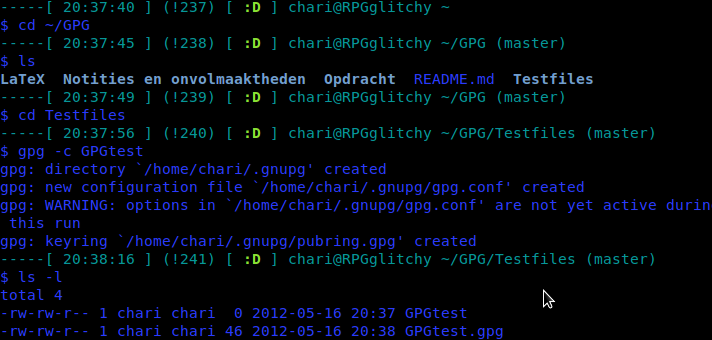
\includegraphics[scale=0.4]{Pictures/terminal}
					\end{center}
					\caption{uitvoer in terminal}
				\end{figure}				
			
			\newpage
			\subsection{Frontend GPG programma's}\label{GUI} 
				\begin{table}[!ht]
					\begin{center}
						\begin{tabular}{r|l}
							Cryptophane	&	Een applicatie voor Windows.\\
							Gajim		&	Een Jabber client voor GNOME.\\
							GnuPG Shell	&	Een cross-platform, grafische Frontend voor GnuPG.\\
							GPA			&	De standaard Frontend voor GPG.\\
							KGpg		&	GnuPG voor KDE.\\
							Seahorse	&	GnuPG voor GNOME.\\
							Wija		&	Een cross-platform jabber client (MacOsX, Linux, 														Windows)\\
						\end{tabular}
					\end{center}
					\caption{Gui Frontends}
				\end{table}

				\begin{figure}[!ht]
					\paragraph{Cryptophane}
						Deze wordt gebruikt om te encrypteren, decrypteren, handtekenen, beheer van 							sleutelhanger en een command-line interface voor GnuPG.\\
					\begin{center}
						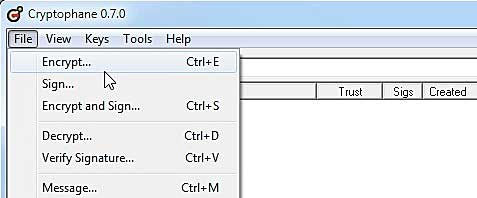
\includegraphics[scale=0.6]{Pictures/cryptophane}
					\end{center}
					\caption{Cryptophane}
				
					\paragraph{Gajim}
						Gajim is een Jabber-client. Een Jabber-client is een messaging applicatie.
						Omdat Gajim werkt met GnuPG, zullen de berichten die verzonden worden met 								Gajim, Geincrypteerd worden.
					\begin{center}
						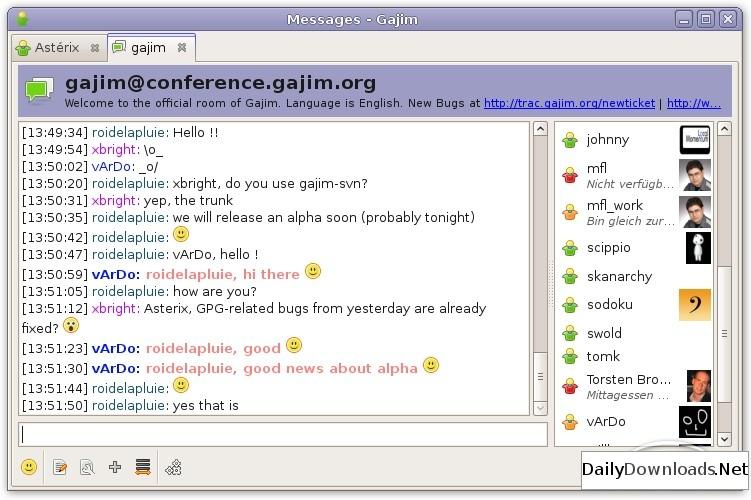
\includegraphics[scale=0.4]{Pictures/gajim}
					\end{center}
					\caption{Gajim}
				\end{figure}
				
				\begin{figure}[!ht]
					\paragraph{GPGshell}
						Een grafische frontend voor iedere platform. Met deze GUI is het mogelijk 								sleutels bij te houden en te encrypteren. 
					\begin{center}
						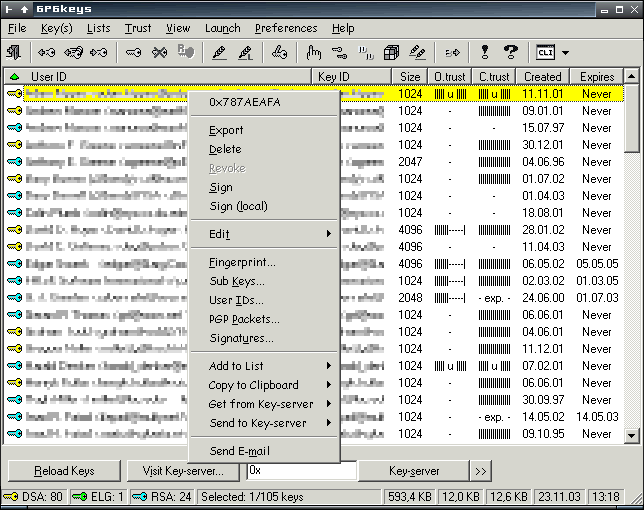
\includegraphics[scale=0.5]{Pictures/gpgshell}
					\end{center}
					\caption{GnuPG Shell}
				
					\paragraph{GPA}
						GPA probeert de standaard frontend te zijn voor GPG. $www.gnupg.org$ Host 								GPA.
					\begin{center}
						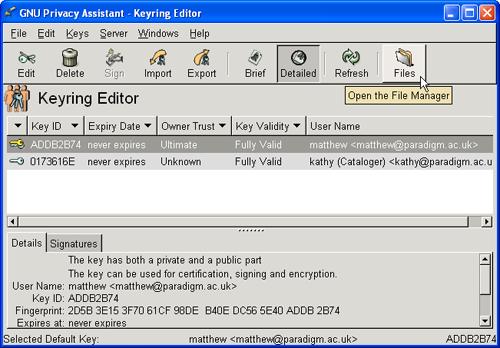
\includegraphics[scale=0.6]{Pictures/GPA}
					\end{center}
					\caption{GPA}
				\end{figure}
				
				\begin{figure}[!ht]				
					\paragraph{KGpg}
						Met KGpg kan je bestanden en mails encrypteren en dycrepteren om je 									informatie veilig te houden.
						Het is een gratis en open-source frontend.
					\begin{center}
						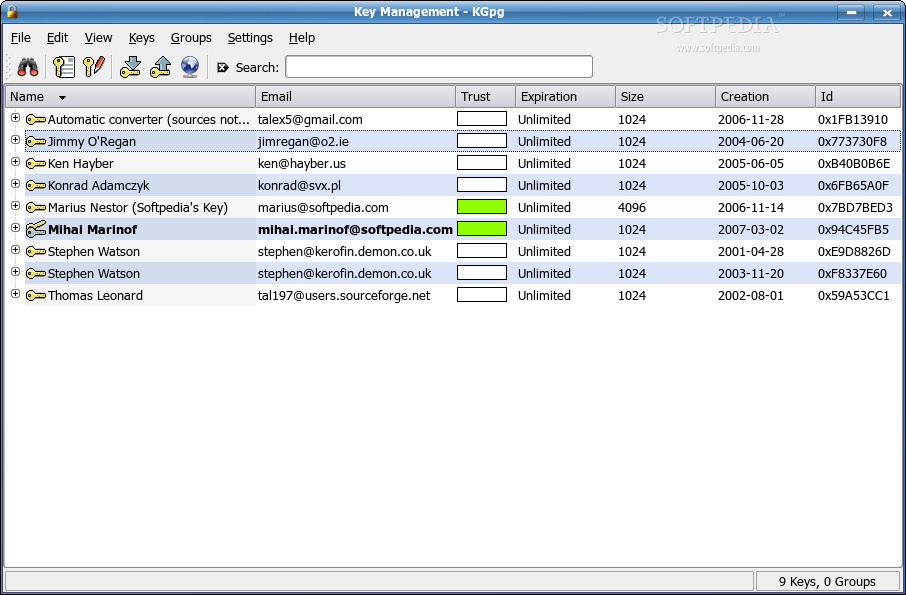
\includegraphics[scale=0.2]{Pictures/kgpg}
					\end{center}
					\caption{KGpg}
				
					\paragraph{Seahorse}
						Seahorse is een GUI voor GNOME. Het is ook geintegreerd in Nautilus, gedit 								en andere applicaties voor encryptie uit te voeren.
						Je kan met Seahorse; PGP en SSH sleutels maken en beheren, publiceren en 								terughalen van sleutels op de servers, een passphrase cachen, 											sleutelhanger backuppen, enz...
					\begin{center}
						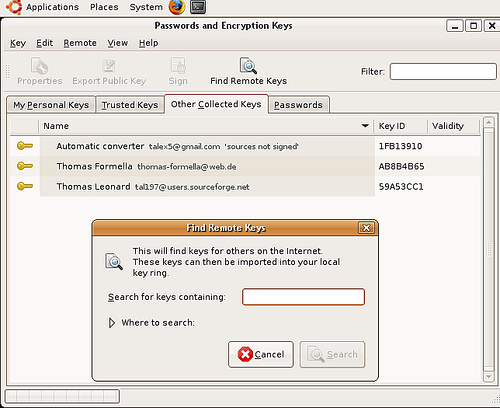
\includegraphics[scale=0.4]{Pictures/Seahorse}
					\end{center}
					\caption{Seahorse}
				\end{figure}
				
				\begin{figure}[!ht]				
					\paragraph{Wija}
						Een Jabber-client zoals Gajim, maar geschreven in java en beschibaar voor 								ieder platform.
						Het heeft een ingebouwde sleutelhanger beheersysteem. Het kan ook zeer 									gemakkelijk boodschappen encrypteren en dycrepteren voor gewone gesprekken of 							multi-user gesprekken.
						Het is ook mogelijk de boodschappen te handtekenen.
					\begin{center}
						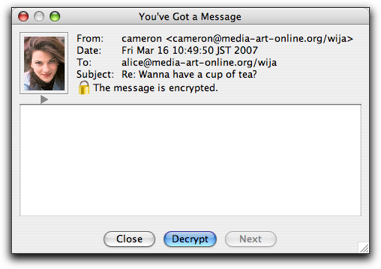
\includegraphics[scale=0.7]{Pictures/wija}
					\end{center}
					\caption{Wija}
				\end{figure}
				
		\subsection{Werking van een GPG Frontend}\label{Frontend}
			Een grafische applicatie voor het gebruik met GPG houdt heel vaak in dat een bestand
			geladen wordt en de gebruiker dan kan kiezen om te encrypteren of decrypteren.\\
			Als de Frontend gebruik maakt van een messaging applicatie (Jabber-client),
			Houdt dit meestal in dat de gebruiker een handtekening instelt in de GUI,
			zodat deze gebruikt wordt bij het encrypteren van de boodschappen.\\
			Als de GUI een sleutelhanger-functie heeft, zal er een instelling van een 'Passphrase'
			Voorzien zijn bij de initieele stappen. Deze passphrase zorgt ervoor dat de sleutelhanger
			ontgrendelt kan worden voor gebruik. Als er dan een wachtwoord wordt ingesteld op een
			website of applicatie, Zal er worden gevraagd deze op te slaan in je sleutelhanger.
			Als de gebruiker dit toestaat, wordt deze geincrypteerd toegevoegd aan je sleutelhanger.
						
		\section{Belangrijke woorden}\label{Belangrijke woorden}
			\begin{table}[!ht]
				\begin{center}
					\begin{tabular}{r|l}
						Jabber-client		&	\\
						Cross-platform		&	\\
						Multi-user			&	\\
						Passphrase			&	\\
						$[!ht]$				&	$h=here, t=top$\\
					\end{tabular}
				\end{center}
				\caption{Belangrijke woorden}
			\end{table}

		\newpage
		\section{Referenties}\label{Referenties}
			$http://www.jumaros.de/rsoft/index.html$ \\
			$http://www.gnupg.org/related_software/frontends.en.html$ \\
			$http://www.google.be$\\
			$http://utils.kde.org/projects/kgpg/$\\
			$http://projects.gnome.org/seahorse/$\\
			$http://tex.stackexchange.com/questions/8652/what-does-t-and-ht-mean$\\
					
	Geschreven door ~\cite{Chari01}
	\bibliography{myBib}{}
	\bibliographystyle{plain}

\end{document}
